\chapter{Empirical Study}
\label{ch:Empirical study}
\lhead{Chapter 4. Empirical Study}

%As described in Section~\ref{sec:rel_works}, there have been some earlier works by the Semantic Web community on building mobile RDF triplestores.
%However, their performance has not been thoroughly evaluated.
%This chapter thus provides an empirical investigation of the performance and storage ability of existing mobile RDF triplestores.
%Based on the experimental results, we analyse the systems' behaviour to see how they are impacted in the context of constrained resources. 
%These findings will serve as input for our design in the following chapter.

%The goals of the case study:
%\begin{itemize}
%    \item positioning the research subject within the IOT field.
%    \item clarify the section motivation.
%    \item defining the requirements for RDF engines on the scenario.
%    \item defining the empirical problem and discuss on the hypothesis $\to$ the approach in the next chapter.
%\end{itemize}

%Hypotheses:
%\begin{itemize}
% \item how the CPU influences the performance
% \item how the Ram influences the performance
% \item how the flash influences the performance
%\end{itemize}

\section{Motivated Scenario}

The scenario is to build up an  IoT system for environmental data management.
Typically, a system for monitoring weather data can be deployed with a three layers architecture(cf. Figure~\ref{fig:4-1-a-centralised}): perception layer, transition layer and data centre layer.
In perception layer, wireless sensors can be placed in territory to collect physical data such as temperature, humility or wind speed.
The collected data can be forwarded to the transition layer using low-range communication technologies such as Zigbee or Bluetooth. 
The transition layer consists of gateway devices that are equipped with wire or wireless long-range communication technologies.
Via transition layer, the data can be sent to the data centre layer in which data is stored and processed.


\begin{figure}[ht!]
    \centering
    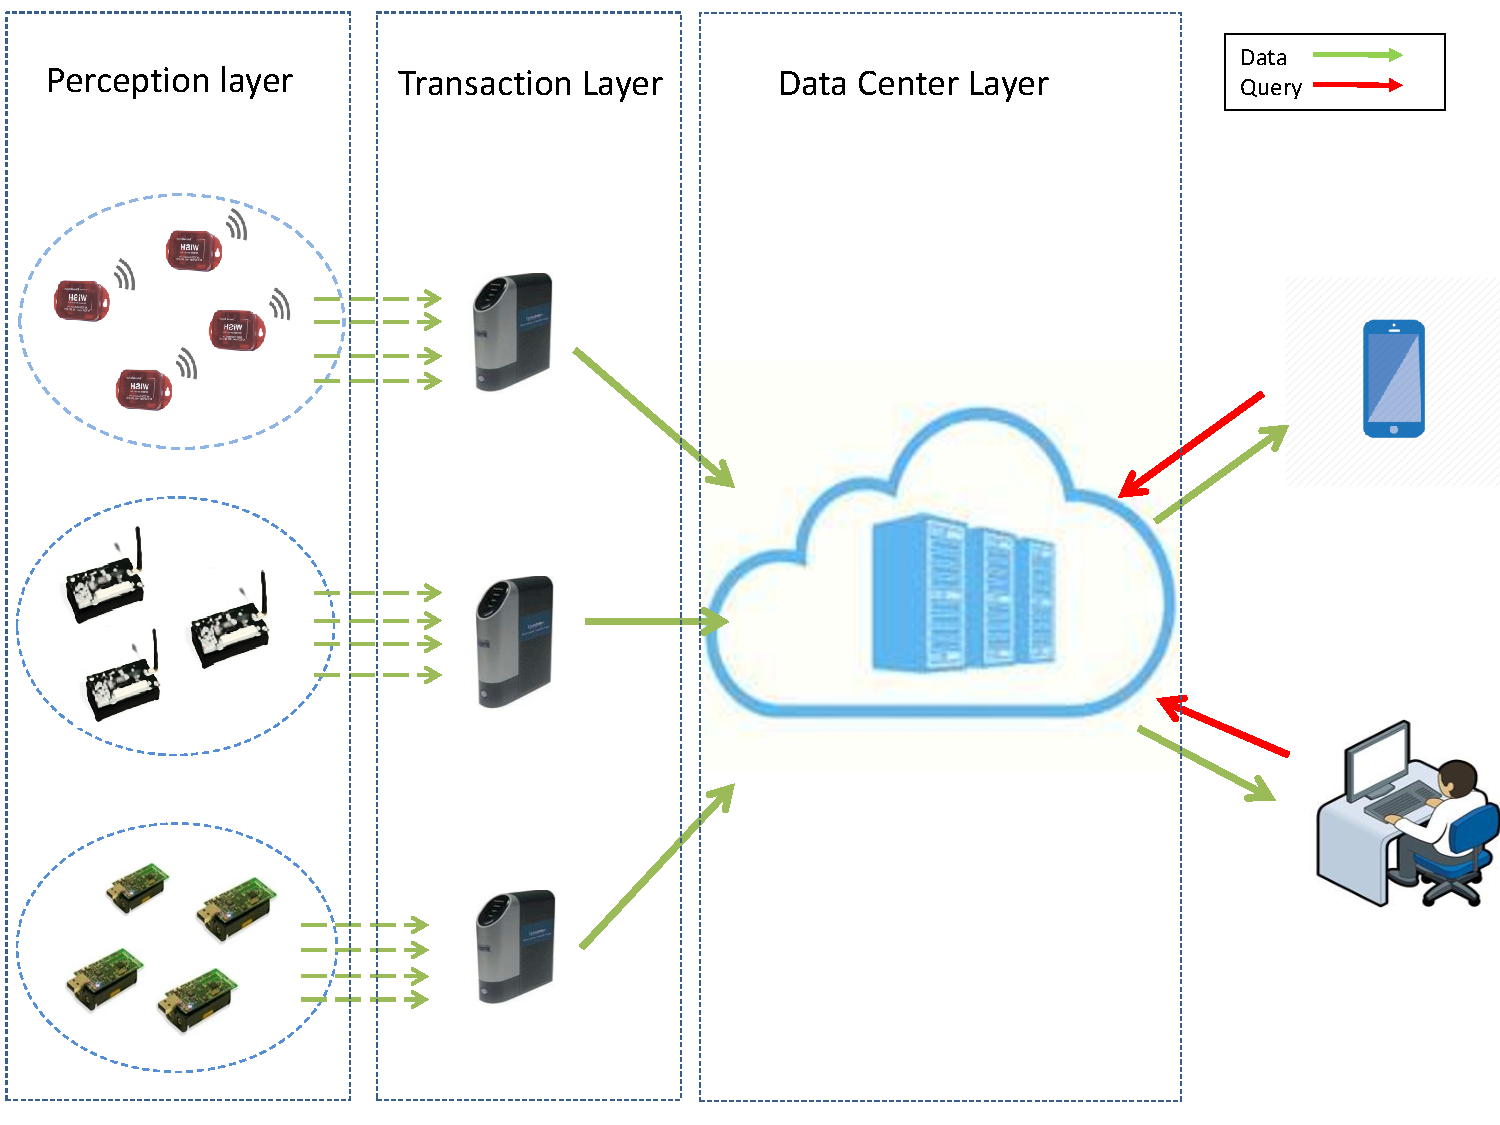
\includegraphics[scale=0.35]{/c4/c4-1-a-centralised.pdf}
    \caption{Architecture of a typical cloud-based IoT system.}
    \label{fig:4-1-a-centralised}
\end{figure}

In contrast to such centralised deployment, an edge-based system aims to push the data processing tasks away from a centralised node.
With the improvement of communication capability of the high-end IoT devices, they can be deployed as gateway nodes in the transition layer. 
Leveraging the advance of storage capability and computational power on such devices, data can be stored and queried from the gateway nodes.

\begin{figure}[ht!]
    \centering
    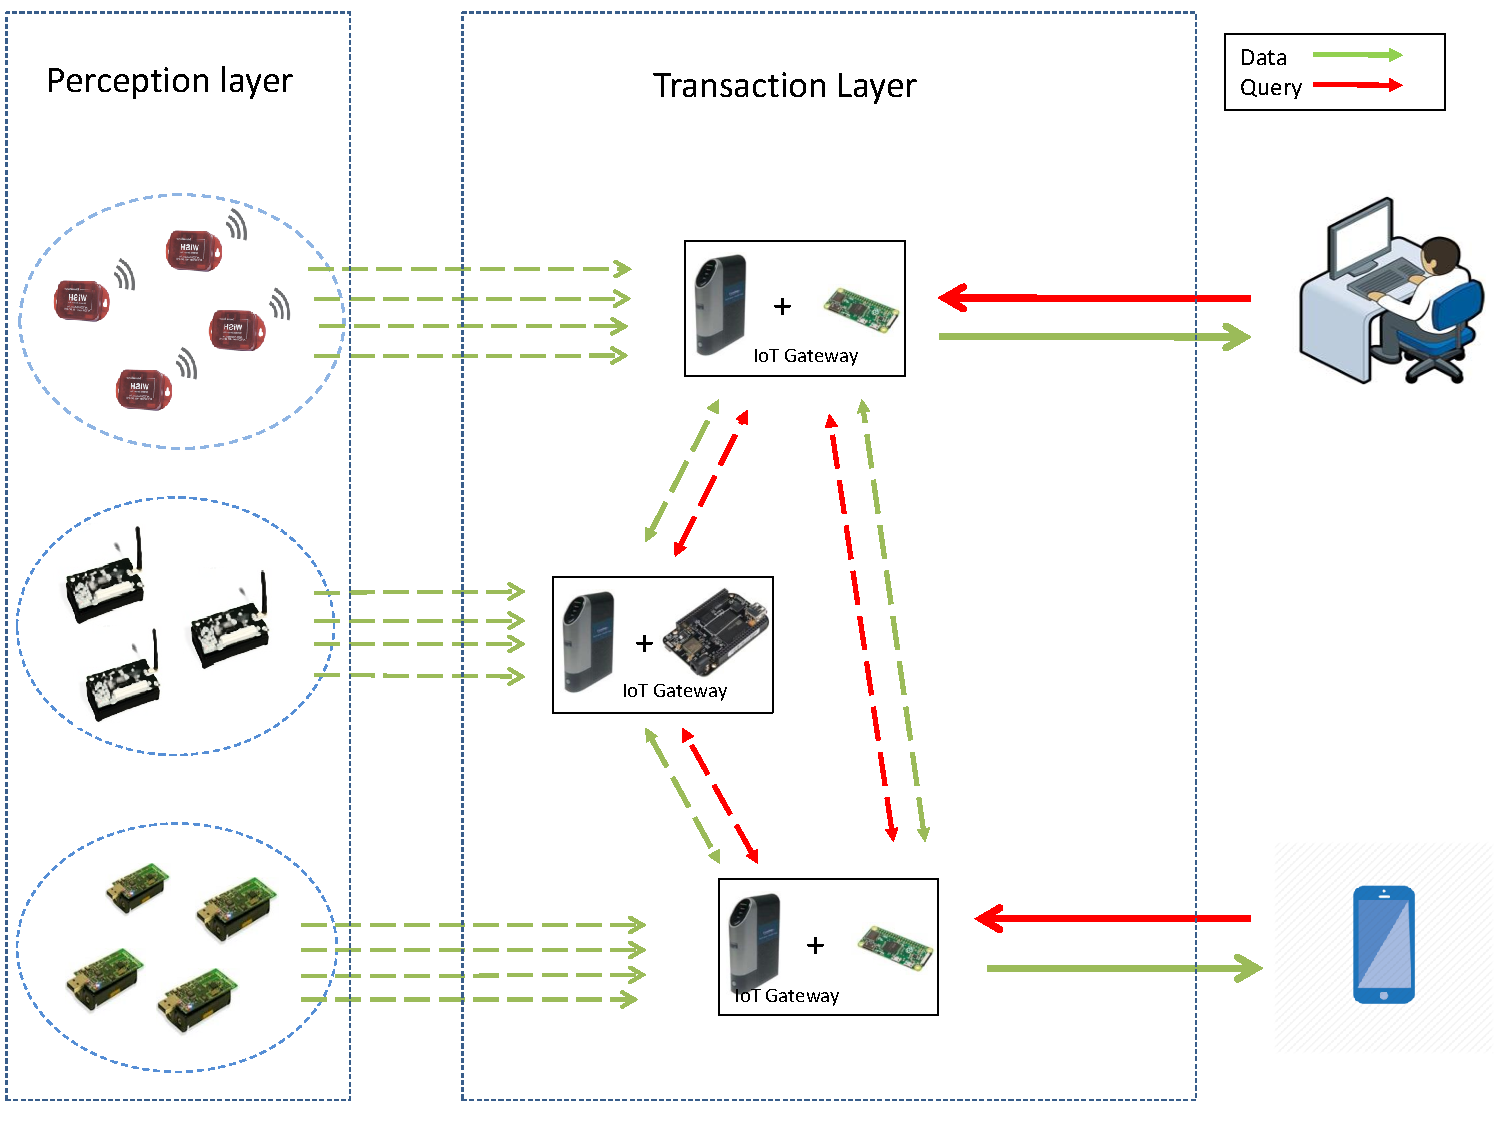
\includegraphics[scale=0.35]{/c4/c4-1-b-decentralised.pdf}
    \caption{Architecture of a typical cloud-based IoT system.}
    \label{fig:4-1-b-decentralised}
\end{figure}

The major challenge of such system is to enable the integration of the sensory data and the data federation between gateway nodes.
The information captured from each sensor device may be presented in a specific scheme, data structure.
Application may require to integrate the collected data which is stored on different gateway nodes.
Therefore, wrapper mediator architecture for data integration can be adopted to provide such integration and federation.
The working principle of such system is quit simple.
A wrapper converts data from specific data sources into objects of a common information model.
Queries from a mediator are transformed to queries understood by the sources and can be sent to other mediators.
The results are collected from the mediators and are merged before returning the answer.

In the scenario, Linked Data technologies is ideally a solution to deal with the heterogeneity of data and data sources.
Similarly to a typical deployment of an IoT system, in the perceived layer, 
the low-end devices (e.g., sensors, actuators) can be deployed across several sites in different locations (e.g., houses or weather stations).
The devices in the same site can be connected to a high-end devices which stand as gateway nodes. 
The RDF engines such as Jena TDB or Virtuoso can be brought to such devices to create such mediators. 
Physical data from low-end devices can be wrapped into RDF data and can be stored on the mediators using an RDF storage.
The federation mechanism of federated SPARQL queries can be also leveraged to provide the integration of mediators.
Simple data model of SPARQL federation such as RDF serialisation or SPARQL result can be used for information exchange between mediators.

\section{Evaluation}

In such edge-based system, the scalability of each edge nodes will contribute to the scalability of the whole system.
The more data can be handle from the edge node, the less likely data has to be sent outward networks.
With the growth of the Semantic Web, there have been many researches for scalable RDF data management.
The cloud-based RDF engines, such as ..., are able to handle billions to trillions of RDF triples.
On the common workstation, the RDF engines such as Jena TDB or BlazeGraph can efficiently store and query RDF dataset of hundreds of millions of RDF triples.
In this study, we aimed to investigate how much RDF data can be handle on the lightweight edge devices.

\subsection{DataSet}

For the evaluation, we used a generated RDF dataset that is similar to the Linked Sensor Data~\citep{}.
The real weather data was taken from the weather data dataset of NOAA's National Centers for Environmental Information(NCEI).
The weather data in this dataset was collected from around 20,000 weathers station in US.
On average, there are five sensors per weather station that measure the phenomena.
In order to describe the data in RDF format we used the updated version of SSN ontology~\footnote{https://www.w3.org/TR/vocab-ssn/}.

\begin{figure}[ht!]
    \centering
    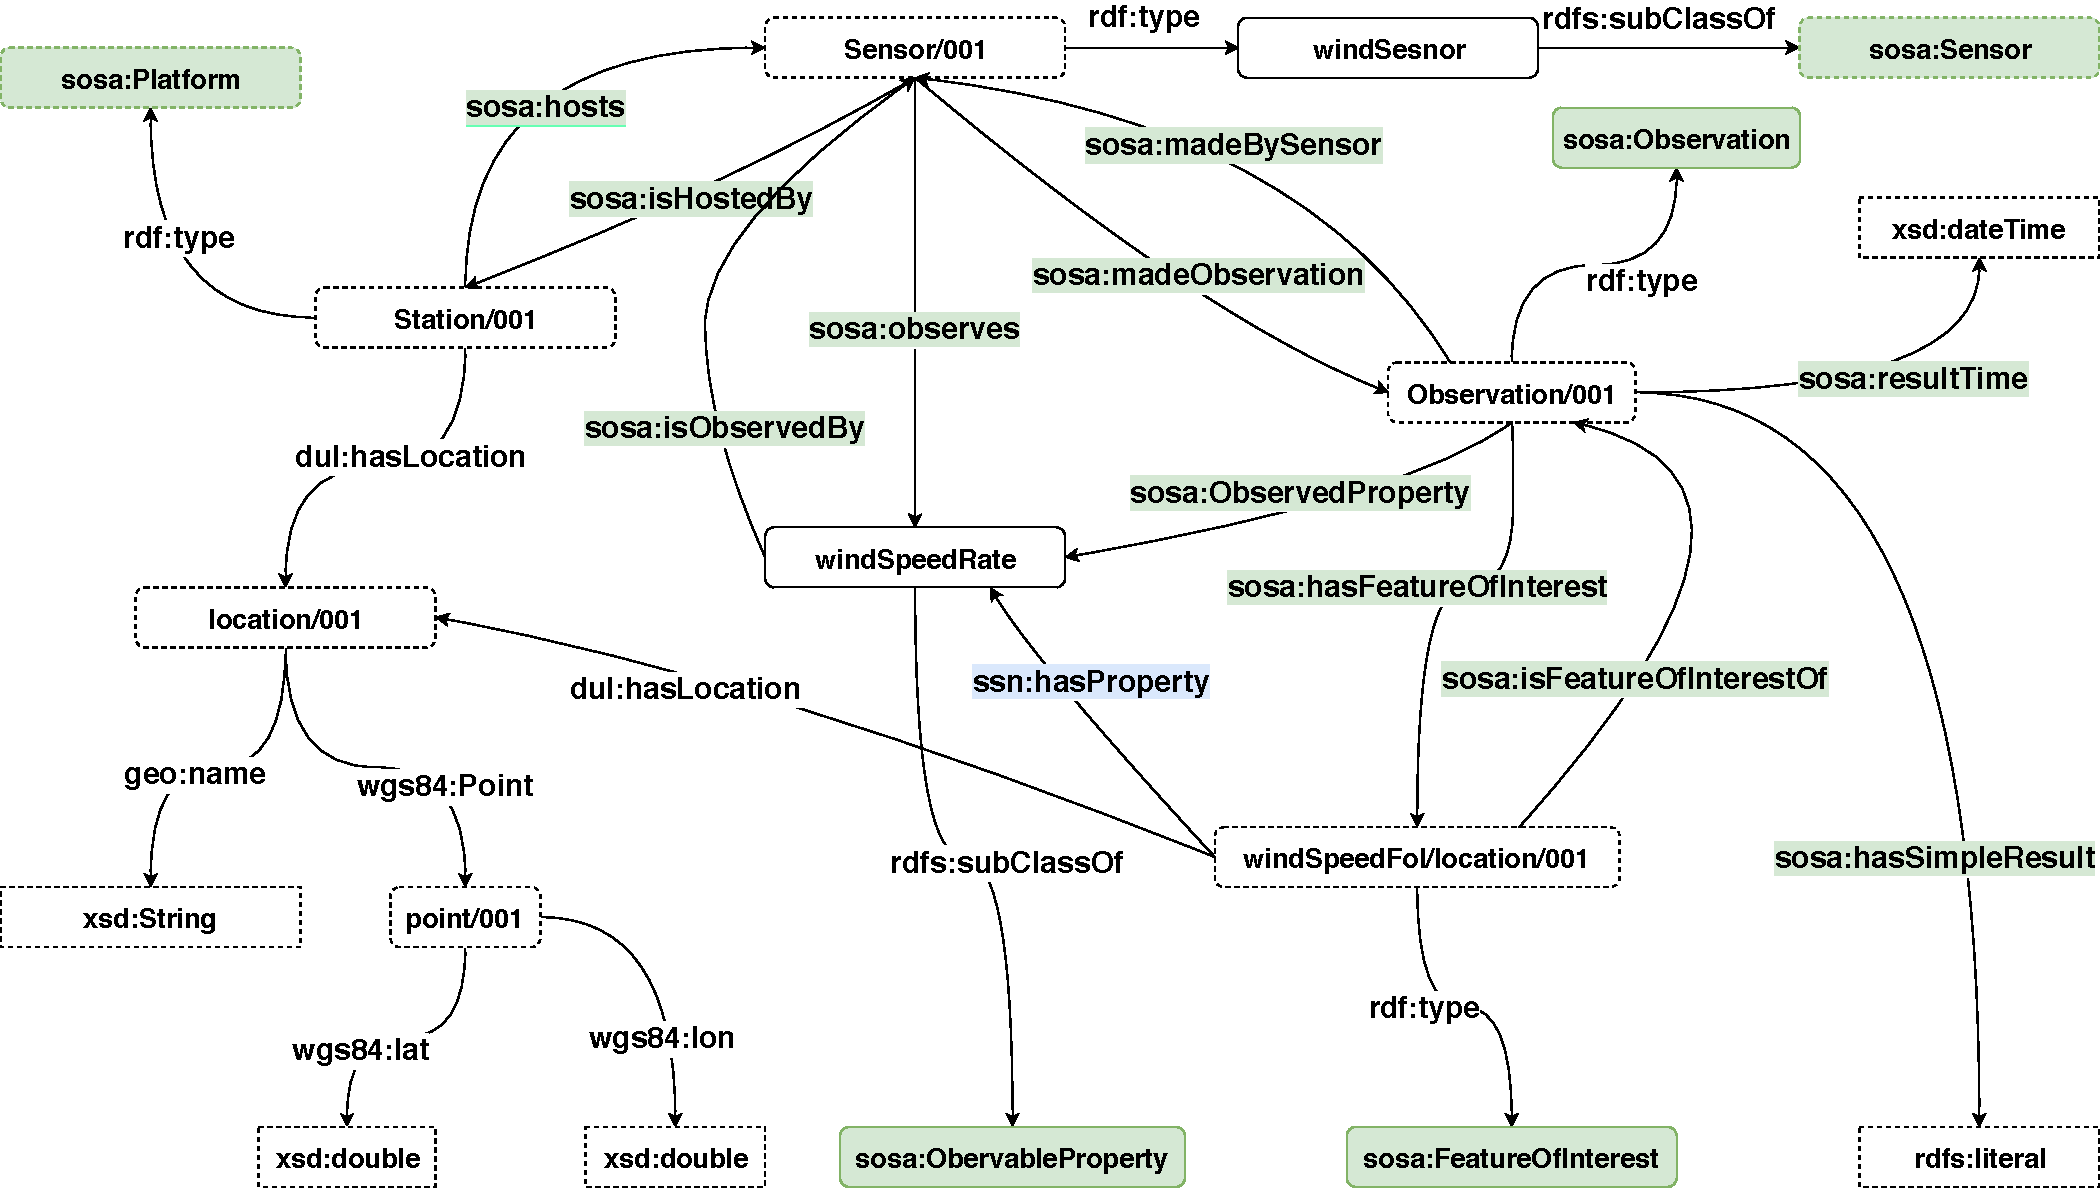
\includegraphics[scale=0.45]{/c4/c4-4-Schema}
    \caption{RDF schema for describing a weather station}
    \label{fig:4-3-weather-station}
\end{figure}

%\begin{figure}[ht!]
%    \centering
%    \includegraphics[scale=0.25]{/c4/c4-3-sensorSchema}
%    \caption{RDF schema for describing a weather station}
%    \label{fig:4-3-weather-station}
%\end{figure}

Figure~\ref{fig:4-3-weather-station} illustrates the RDF schema that describes a weather station.
Each weather station is represented by an URI and is defined as a system using \textbf{rdf:type} property and \textbf{ssn:System} class.
In consequence, a weather station has five sensors which are linked with the weather station using property \textbf{ssn:hasSubSystem}.
Each sensor has type \textbf{sosa:Sensor} and observes a specific \textbf{sosa:ObservableProperty}.
In addition to location attributes of weather station such as latitude, longitude, and geonames are also provided using GeoNames~\footnote{http://www.geonames.org/ontology/documentation.html} and WGS84~\footnote{https://www.w3.org/2003/01/geo/}.

The observations collected include measurements of phenomena such as temperature, visibility, precipitation, pressure, wind speed, humidity. 
The weather station’s observations also include the unit of measurement for each of these phenomena as well as the time instant at which the measurements were taken. 
The RDF schema that describes an observation, specifically wind speed, is illustrated in Figure~\ref{fig:4-3-observation}.
Each observation is linked to the sensor that made this observation using \textbf{sosa:madeObservation} and \textbf{sosa:madeBySensor}.
The phenomena is defined by the \textbf{sosa:FeatureOfInterest} class.
The observation is linked to its feature of interest using property \textbf{sosa:hasFeatureOfInterest} and \textbf{sosa:isFeatureOfInterestOf}. 
For example, the wind speed observation URI is connected to \textbf{windSpeedFOIIRI}.
The measurement unit of an observation is an plain literal, and time stamp of an observation is type literal.
They are connected to the observation using properties \textbf{sosa:hasSimpleResult} and \textbf{sosa:resultTime} perspectively.


%\begin{figure}[ht!]
%    \centering
%    \includegraphics[scale=0.35]{/c4/c4-4-observationSchema}
%    \caption{RDF schema for station metadata}
%    \label{fig:4-3-observation}
%\end{figure}

The example of using SPARQL query that extracts data from the sample dataset is presented in listing~\ref{lst:sparql_q1}.
The query is to request all wind speed measurement from station 1. 
The rest of the queries that are used in the experiment can be found in Appendix~\ref{}.

%====================================================================================
\begin{lstlisting}[
captionpos=b, 
language=sparql,
label={lst:sparql_q1},
basicstyle=\scriptsize\ttfamily,
caption={List all the wind speed values from a given station and order by time}]
PREFIX ssn:<http://www.w3.org/ns/ssn/>
PREFIX sosa:<http://www.w3.org/ns/sosa/>
PREFIX insight:<http://insight.org/dev/noaa/>

SELECT ?windSpeed ?time
WHERE
{
    insight:Station1 sosa:hasSubSystem ?sensor.
    ?sensor a sosa:Sensor.
    ?sensor sosa:madeObservation ?observation.
    ?observation sosa:hasFeatureofInterest insight:windSpeedFOIIIRI.
    ?observation sosa:resultTime ?time.
    ?observation sosa:hasSimpleResult ?windspeed.
}
ORDER BY (?time)
\end{lstlisting}


The measurements were read every half an hour and it is required 80 RDF triples to describe a measurement.
In order to store the data of a weather station in a year in active RDF graph on a gateway node, the RDF engine that runs on this node needs to store up to 1.5 millions RDF triples.
The dataset we used in the experiment was wrapped data from 20 workstation in year 2017.
The size of the dataset is 30 million triples.

\subsection{Hardware devices}

The experiments were conducted on three types of high-end IoT devices: Intel Galileo Gen II(GII), Raspberry Pi Zero W (Pi0), and Beagle Bone Black(BBB).
We chose these devices because they were popular and have been used for demonstrating the proof of concept of many researches in the IoT domain.
Furthermore, they are representatives for resource barriers of IoT gateways in our scenario in terms of size, memory and cost.

The Intel Galileo was developed by Intel and was the first IoT device that can run a complete Linux system.
The Intel Galileo was designed as hardware and software Arduino-compatible.
The design allowed Arduino sensors and actuators can be used out of the box on Galileo. 
Therefore, the Galileo hardware can be thought as composed by two set of hardware components which are the Arduino hardware and the "mini PC" hardware.
The Intel Galileo was equipped with RAM, Flash memory, mini SD card reader and Ethernet adapter.
Differently from the other boards, the Intel Quark x86 CPU was embedded on the board instead of the ARM CPU family.
Galileo came out with two versions: the Gen 1 Intel Galileo  and the Gen 2 Intel Galileo.
They are pretty similar, however, the Gen 2 boards had some hardware improvements.
Thus, we only use Galileo Gen 2 in our evaluation.

BeagleBoard was originally developed and introduced by Texas instruments in year 2008.
By using OMAP3530 System-on-a-chip technology, BeagleBoard boards were good platform to various demonstrating scenario in the researches of the IoT.
It was regarded as giant step that bring the microcontrollers to the full-fledged microcomputer. 
BeagleBone Black was a small credit card-sized BeagleBoard that was launched in 2013 at a price of $\$$45. 
Among other differences, on BeagleBone Black RAM was increased to 512 MB, ARM Cotex-A8 processor with the processor clock up to 1 GHz was equipped, and there was also 2 GB of eMMC flash memory on this small board. 

The Raspberry Pi was another the well-known, low-cost single board computer that was developed by the University of Cambridge.
Today, Raspberry Pi’s capabilities are similar to a PC, as it allows browsing the Internet, playing games, playing HD videos, working with word processing and spreadsheet applications. 
The Raspberry Pi is able to acquire information from sensors and interact with the actuators. 
The current models of Raspberry Pi are Model A+, Model B+, Pi 2 Model B and Pi Zero.
A Raspberry Pi Zero with smaller size  was released in 2015.
In 2017, the Raspberry Pi Zero W was launched, a newer version of the Zero with Wi-Fi and Bluetooth capabilities, for US$\$$10.
The Raspberry Pi runs Raspbian (a free operating system based on Debian Linux and optimized for the Raspberry Pi hardware). 

The configurations of each device are summarised on table~\ref{t:hc}. 

\begin{table}[ht!]
\centering
\begin{tabular}{ c | p{3.5cm} | p{3.5cm} | p{3.5cm} |}
\cline{2-4}
& \multicolumn{3}{c|}{Devices} \\  
\cline{2-4}
                                    & \multicolumn{1}{c|}{Pi0} & \multicolumn{1}{c|}{BBB} & \multicolumn{1}{c|}{GII}\\ 
\hline
\multicolumn{1}{|c|}{CPU}          & \multicolumn{1}{c|}{ARM 11,    1.0 GHz, 1-core }
								   & \multicolumn{1}{c|}{ARM A8,    1.0 GHz, 1-core }
                                   & \multicolumn{1}{c|}{x86 Quark, 0.4 GHz, 1-core } \\
\hline
\multicolumn{1}{|c|}{RAM}          & \multicolumn{1}{c|}{512 MB} & \multicolumn{1}{c|}{512 MB} &\multicolumn{1}{c|}{256 MB} \\
\hline
\multicolumn{1}{|c|}{Storage}      & \multicolumn{3}{c|}{Transcend MicroSD 16GB class 10 (40MB/s)} \\
\hline
\multicolumn{1}{|c|}{OS}           & \multicolumn{1}{c|}{Raspbian} & \multicolumn{1}{c|}{Debian 7.0} & \multicolumn{1}{c|}{Yocto} \\
\hline
\end{tabular}
\caption{Hardware Configurations}
\label{t:hc}
\end{table}

\subsection{RDF engines}
We run the experiment with three RDF engines that were able to set up on the three targeted devices: Jena TDB, Sesame, and Virtuoso.

Jena TDB is a component of Apache Jena, a Semantic Web framework that is available as open-source software.
Jena TDB is the persistent storage layer for Jena, and it works with Jena SPARQL query engine (ARQ) to provide complete SPARQL.
Jena TDB is a pure-Java implementation, employing memory mapped I/O, a custom implementation of B$^+$Trees.
TDB was tested with UniProt v13.4 (1.7B triples, 1.5B unique) on a single machine with 64 bit hardware.
It performed loading an average 12 thousands of triples per second.
In the experiment, Jena TDB version 3.5 was used.

Sesame is another Java-based open source framework for storage, inferencing and querying of RDF data.
Sesame includes RDF parsers and writers (Sesame Rio), a repository API for handling RDF data. 
It operates in any Java-supporting environment and can be used by any Java application.
Sesame provides native as well as RDB-backed triple storage. 
Sesame with ... was used.

Virtuoso is developed by OpenLink Software Inc, and it is a hybrid storage solution for a range of data models, including relational data, RDF and XML, and free text documents. 
Virtuoso has a RDB-backed storage, thus, it can be seen as an SPARQL-to-SQL solution for managing RDF data.
Virtuoso has gained significant interest since it is used to host many important Linked Data sets (e.g., DBpedia).
Virtuoso is offered as an open-source version and commercial version.
In this evaluation, we used Virtuoso 6 open-source version because Virtuoso 7 with column store was not able to be installed on 32-bit OS.

\subsection{Experiments}

We run three experiments to monitor the update throughput as we assume weather data should be collected in a sort interval of time, the query response time, and the memory consumption as memory is critical resource in such limited memory devices. The details of each experiment is presented as following:

{Exp1 - Update throughput:}
In the first experiment, we test how much new data the system can incrementally update with a certain underlying RDF store corresponding to each hardware configurations. 
We simulate the process of data growing by gradually adding more data to the system.
The metadata of 20 weather stations was inserted first and then the observation data.
We measure the throughput of inserting data (triples/second) until the system crashes or until the throughput is below 80 triples/second (whichever happened first).
When the system can not insert 80 triples/second, that means the system can not update 1 reading in a second.

{Exp2 - Query evaluation:} 
In the second experiment, we test the queries response time of each engine.
On each device, we chose the size of the dataset with the scale that all the engines can store.
We followed the approach of WATDIV benchmark to create queries with different shapes: linear, star or snowflake.
The set of queries can be found in the Appendix~\ref{}.
We recorded the maximum, the minimum and the average time that the engines answer each type of queries.

{Exp3 - Memory consumption:}
In the third experiment, we measured the memory consumption of three system configurations while performing the insertion and query.  
The experimental application ran the different queries repeatedly and recorded the maximum memory heap that the operating system allocated for it. 
Note that the memory consumption is device-independent. 
To evaluate the impact of the data size on memory consumption, the test was conducted on the BBB with 15 datasets and with different sizes.dataset. 
The scale ranges from 2 million triples to 50 million triples. 

\section{Result}

\subsection{Insert Throughput}


\newpage

\begin{figure}[ht!]
    \centering
    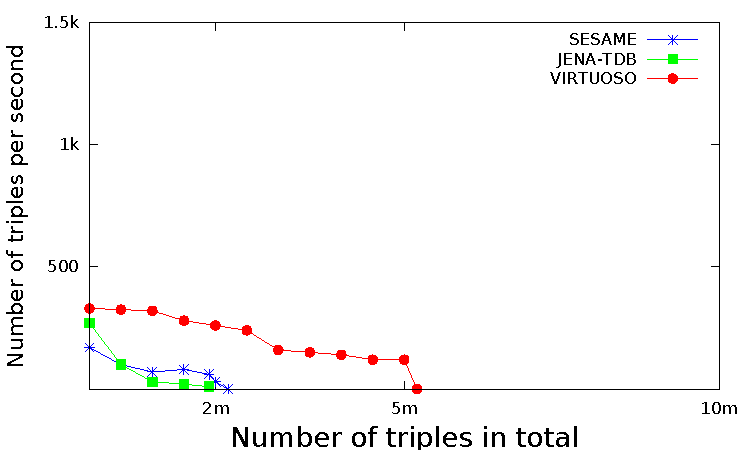
\includegraphics[scale=.85]{/c4/c4-GII-input}
    \caption{Insert throughput on Gallileo Gen II}
    \label{fig:4-3-GII}
\end{figure}

\begin{figure}[ht!]
    \centering
    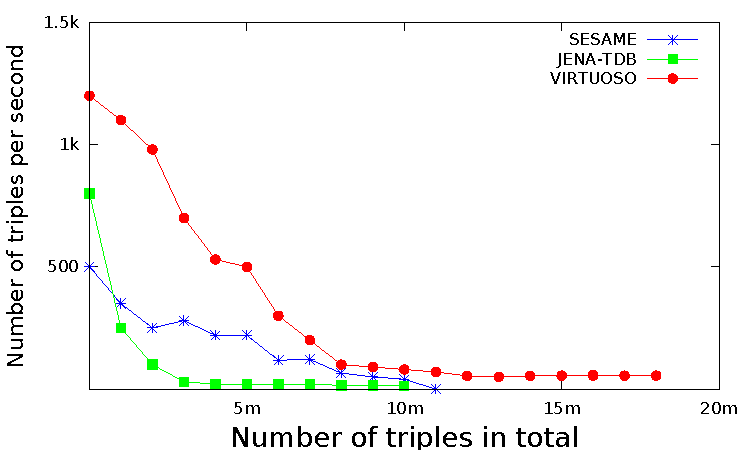
\includegraphics[scale=.85]{/c4/c4-BBB-input}
    \caption{Insert throughput on BeagleBone Black}
    \label{fig:4-3-BBB}
\end{figure}

\begin{figure}[ht!]
    \centering
    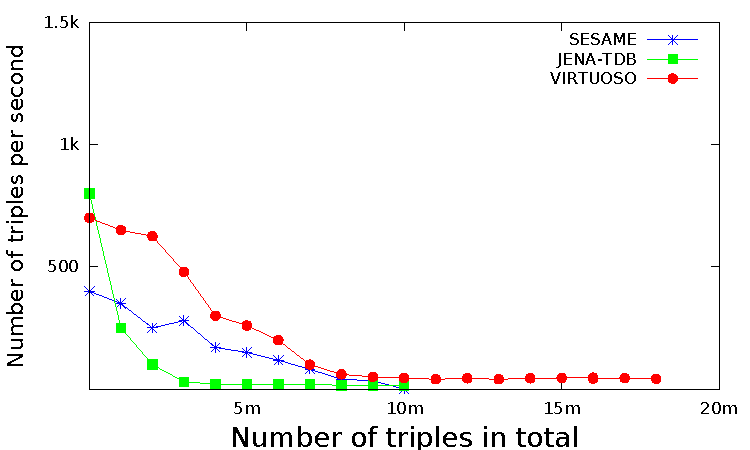
\includegraphics[scale=.85]{/c4/c4-PI0-input}
    \caption{Insert throughput on Raspberry Pi Zero}
    \label{fig:4-3-PI0}
\end{figure}
\newpage


\subsection{Query Response Time}

\newpage
\subsection{Memory Consumption}

\begin{figure}[ht!]
    \centering
    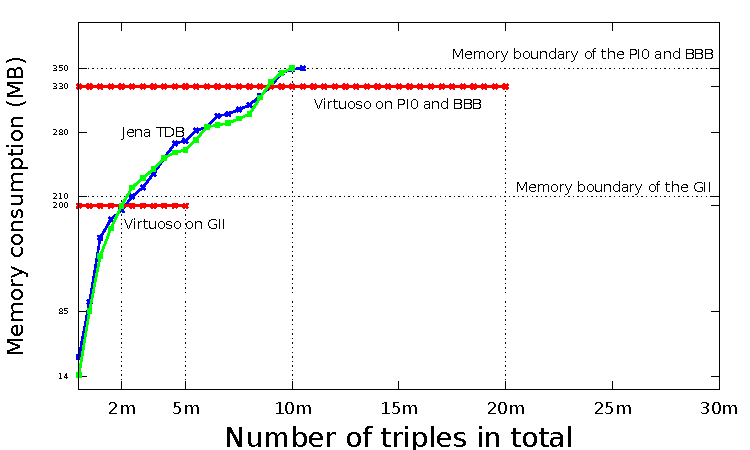
\includegraphics[scale=.85]{/c4/c4-input-mem}ifc
    \caption{Insert throughput on BeagleBone Black}
    \label{fig:4-3-BBB}
\end{figure}

\begin{figure}[ht!]
    \centering
    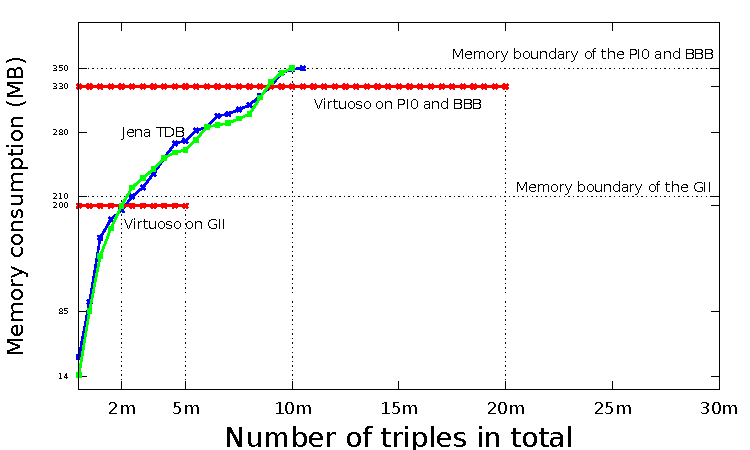
\includegraphics[scale=.85]{/c4/c4-query-mem}
    \caption{Insert throughput on Raspberry Pi Zero}
    \label{fig:4-3-PI0}
\end{figure}
\newpage

\section{Discussion}























